\section{Results and Discussion}

This section summarizes the results obtained from the Halo Assay, BS Assay, and Jar Assay, focusing on bacterial interactions, fungal inhibition, and plant growth effects.

\par
The first set of data analyzed focused on the effects of different bacterial strains on the root weight and root length of barley plants. These results are visualized in \autoref{fig:root_weight_boxplot} and \autoref{fig:root_length_boxplot} respectively.
Both figures are sorted by the mean of the root weight to enable better comparison. 


\begin{figure}[H]
    \centering
    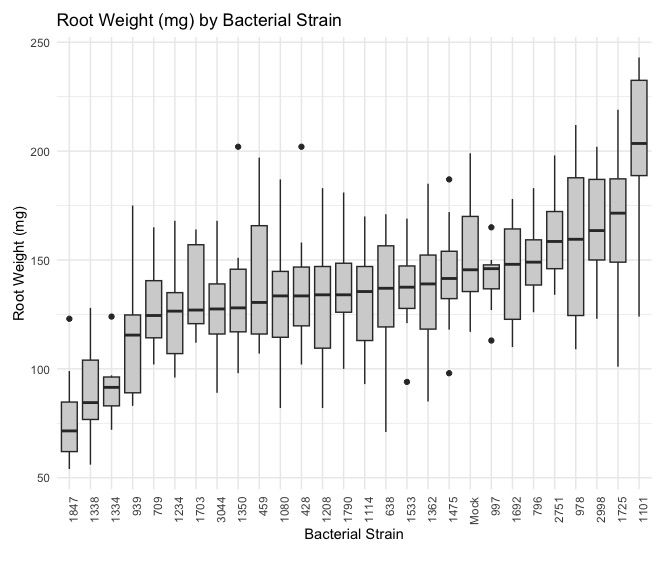
\includegraphics[width=0.8\linewidth]{Figures/Root Weight.jpeg}
    \caption{Root weight of barley after bacterial treatment.}
    \medskip
    \textbf{Description:} Distribution of root weight (in mg) for barley plants treated with different bacterial strains, sorted by the median root weight.
    \label{fig:root_weight_boxplot}
\end{figure}% Root Length Boxplot

\begin{figure}[H]
    \centering
    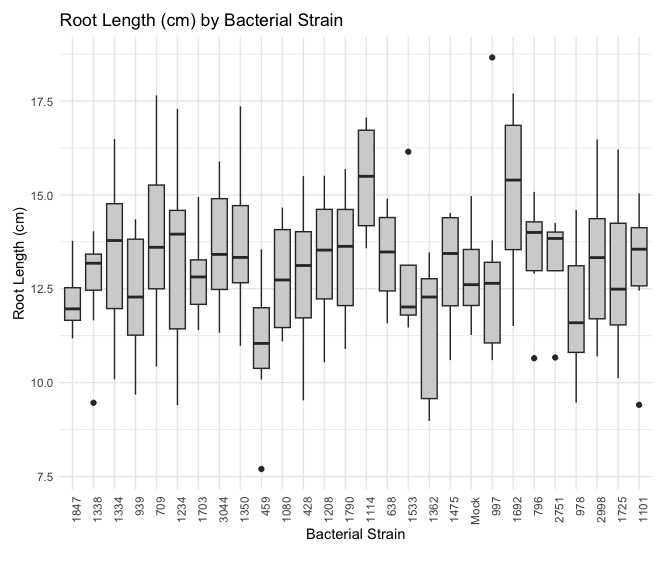
\includegraphics[width=0.8\linewidth]{Figures/RootLength.jpeg}
    \caption{Root length of barley after bacterial treatment.}
    \medskip
    \textbf{Description:} Distribution of root lengths (in cm) for barley plants treated with different bacterial strains, sorted by the median root weight.
    \label{fig:root_length_boxplot}
\end{figure}


The interactions between the bacterial strains, that were evaluated using the Halo Assay are visualized in \autoref{fig:heatmap} in the form of a heatmap. 
This heatmap represents the antagonistic effects observed between bacterial strains, where the size and color of the dots correspond to the size and strength of the inhibition halos, respectively. Small gray dots indicate the absence of halo, despite of bacterial growth, while the absence of a dot indicates no bacterial growth in that interaction. 

Some bacterial strains stood out by producing notably larger inhibition halos, indicating strong antagonistic effects. Most notably, strains 1208, 1847 consistently generated the largest halos, suggesting an ability to inhibit the growth of other strains. These strains displayed both substantial halo size and high halo strength, as represented by darker colors in \autoref{fig:heatmap}.

Certain bacterial strains were unable to establish growth when interacting with any of the other strains, as indicated by the absence of dots in \autoref{fig:heatmap}. This suggests that these strains were either highly sensitive to antagonistic effects from other strains or lacked the competitive ability to survive in such interactions under the experiment conditions. 
For example, strains 1114 and Y showed growth in only a few cases without producing measurable halos, suggesting a neutral or non-antagonistic role within the community.
% Heatmap
\begin{figure}[H]
    \centering
    \raggedright
    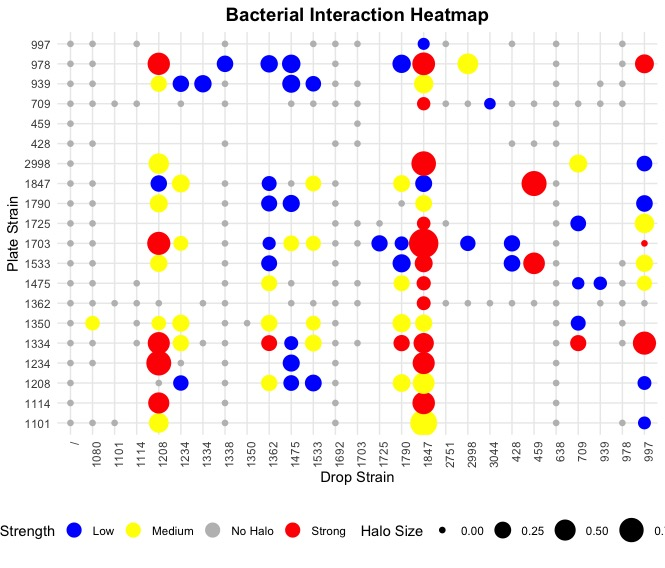
\includegraphics[width=\linewidth]{Figures/Heatmap.jpeg}
    \caption{Bacterial interaction heatmap}
    \medskip
    \textbf{Description:} Heatmap visualizing the interactions between bacterial strains, with halo size and strength indicating antagonistic effects. Grey dots represent no observed halo while the absence of a dot indicated no bacterial growth.
    \label{fig:heatmap}
\end{figure}

\begin{figure}[H]
    \centering
    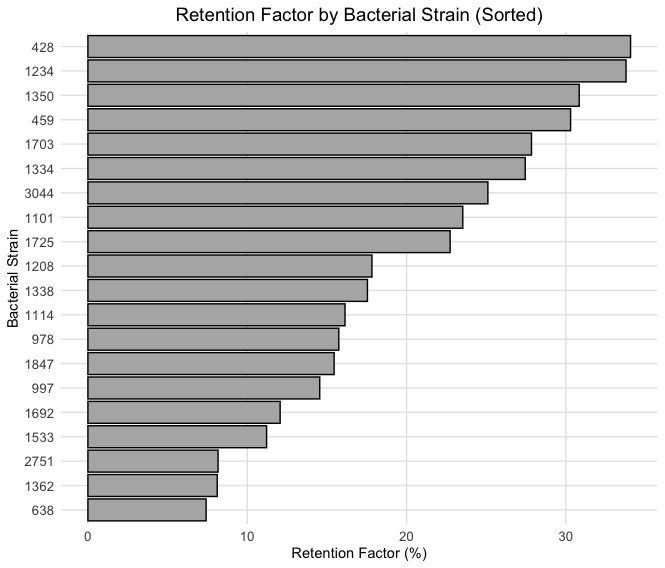
\includegraphics[width=\linewidth]{Figures/RetentionFactor.jpeg}
    \caption{Retention Factor by Bacterial Strain.}
    The retention factor measures the degree of inhibition caused by bacterial strains. 
    See the text below for details on the calculation.
    \label{fig:retention}
\end{figure}

\vspace{0.5cm} % Add space between the figure and the detailed explanation

\noindent
The retention factor is calculated using the formula:
\[
\text{Inhibition (\%)} = \frac{\text{Control Distance} - \text{Bacteria Distance}}{\text{Control Distance}} \times 100
\]
where the \textit{Control Distance} refers to the growth measurement in the absence of bacterial interference, and the \textit{Bacteria Distance} refers to the growth measurement in the presence of bacterial strains. Higher retention factor values indicate greater inhibition by the bacterial strain. The bar plot in \autoref{fig:retention} visualizes the retention factors for each bacterial strain, highlighting differences in inhibitory effects across strains.


Strain 1847 that was classified via the Type Strain Genome Server (TYGS), as can be seen in \autoref{tab:strains}, as \textit{Pseudomonas chlororaphis} conistently showed strong result across the three assay. This indicates a significant antagonistic avtivity towards other strains, effective inhibition of \ac{Bipo} growth and a notable influnce on root growth in the Jar Assay.

This strain was already subject of a study published in 2021 by Bertani et. al., showing several effect both on plant's and fungi. 
In the study, the \textit{Pseudomonas chlororaphis} strain effectively inhibited fungal pathogens like \textit{Fusarium graminearum} through antimicrobial production and colonized plant roots, enriching beneficial microbes in the rhizosphere. While it influenced plant stress pathways, it showed no direct growth-promotion effects under the tested conditions. \cite{bertani2021Isolation}

This correlated with our finings, as the strain reduced plant root growth and length while demonstrating  strong antagonistic effects on other bacterial strains and weak antagonistic effects on the fungal pathogen.